\documentclass{article}
\usepackage[final]{nips_2017}
\usepackage[utf8]{inputenc} % allow utf-8 input
\usepackage[T1]{fontenc}    % use 8-bit T1 fonts
\usepackage{hyperref}       % hyperlinks
\usepackage{url}            % simple URL typesetting
\usepackage{booktabs}       % professional-quality tables
\usepackage{amsfonts}       % blackboard math symbols
\usepackage{nicefrac}       % compact symbols for 1/2, etc.
\usepackage{microtype}      % microtypography
\usepackage{graphicx}
\usepackage{float}
\title{Make yourself into a work of art}

\author{
  Kiah Hardcastle \\
  Neuroscience PhD Program \\
  Stanford University\\
  \texttt{khardcas@stanford.edu} \\
  %% examples of more authors
   \And
  Julie Makelberge \\
  Graduate School of Business \\
  Stanford University \\
  \texttt{juliemkb@stanford.edu} \\
  %% \AND
  %% Coauthor \\
  %% Affiliation \\
  %% Address \\
  %% \texttt{email} \\
  %% \And
  %% Coauthor \\
  %% Affiliation \\
  %% Address \\
  %% \texttt{email} \\
  %% \And
  %% Coauthor \\
  %% Affiliation \\
  %% Address \\
  %% \texttt{email} \\
}

\begin{document}
% \nipsfinalcopy is no longer used

\begin{center}

\includegraphics[width=3cm, height=0.7cm]{CS230}
\end{center}

\maketitle

\begin{abstract}
In this paper, we present a method by which one can integrate a person's face into an artistic painting containing a face. For example, given a headshot and an artistic portrait, this method will inpaint the face in the headshot photo into the portrait face, while retaining the artistic style of the painting. To accomplish this task, we drew upon existing techniques of face swapping and portrait-specific neural style transfer. This approach builds on this previous work in several ways. First, while a number of applications have focused on face swapping in recent years, they have generally been applied to photograph images with a similar style. Second, the few methodologies that have used neural style transfer combined with face-swapping have transfered the transfered the style of the artistic image to the headshot image, without putting the newly-styled headshot image into the artistic image. Thus, our approach is novel in that we aim to retain the style and pose of the original work of art's face, regardless of the pose of the supplied image, and  reintroduce the face in the work of art as a whole. 
\end{abstract}

\section{Introduction}  
With the advent of neural style transfer in 2015 \cite{gatys2015neural}, and generative adversarial networks in 2014 \cite{gan2014}, altering artwork, or even generating novel artwork, via neural networks has become a topic of high interest in both the computer science and art communities. For example, in October 2018, an AI-generated piece of artwork sold for nearly half a million dollars. Over the last year, AI-generated art was featured in art galleries in San Francisco ("DeepDream") and New York City ("Faceless Portraits Transcending Time"). Understanding how neural networks can alter or generate art will be an important component of understanding how AI performs activities previously thought to be restricted to humans. Here, we aim to understand and implement these techniques in order to alter an existing previous piece of artwork in a personalized manner. 

In our method, we alter an existing piece of artwork by injecting the content of a headshot photograph into an original piece of art. Specifically, our framework takes two images: 1. a photograph image containing a face and 2. an artistic photo containing a face, and returns one image: a new version of the original artistic photo, but with the face replaced. The replaced face is in the same pose, and in the same style, as the original artistic face, but the content of the face is drawn from the photographed face. To accomplish this task, we initially thought of using a generative adversarial network, but were encouraged the TA to combine methods of face-swapping with neural style transfer techniques. We believe this combined technique would be valuable in the world of generative art as it allows different and personalised renderings of the same types of art work. 

\section{Related work}

In our project, we implement neural style transfer (NST) to imbue the face in the photograph image with the texture of the artistic photo. NST is the technique of using deep neural networks to transfer the style of a given reference image to the content of another. Prior to 2015, style transfer was accomplished with classic image processing techniques such as histogram matching \cite{neumann2005color}. However, in 2015, Gatys et al. introduced a novel technique that leverages the power of Convolutional Neural Networks (CNN) to emulate famous painting styles in natural images \cite{gatys2015neural}, \cite{gatys2016}. In their seminal paper, they proposed to capture the style and content elements of images by using the activations of different layers of a pre-trained CNN. In many modern works, including this project, VGG-19 is used \cite{Simonyan14c}. 

Their work has inspired a number of new neural transfer algorithms, ranging from general models such as the work of Li and Wand \cite{li2016combining} that combined generative Markov random field models with deep convolutional neural networks, to highly specialized domain-specific models such as Jiang and Fu's Fashion style generator \cite{jiang2017fashion}. While general models have shown great potential in a large number of applications, they generally introduce visual artifacts in faces. Several works have attempted to address these artifacts. In 2014, Shih et al., developed an approach that transfered style between headshot portraits by first finding a pixel-to-pixel correspondence between images, and then decomposing each image into "Laplacian stacks" that they match between images \cite{Shih2014}. However, this method only works between photographs. In 2016, Selim et al. introduced an approach that first aligns the artistic and photograph faces, and then learns a new image via NST with an altered set of content activations \cite{selim2016painting} (described in detail below). This technique works well for portrait-specific NST, but does not replace the face in the artistic image. In 2017, Liao et al. developed another approach using "deep image analogy" \cite{Liao2017}. Briefly, this approach takes two semantically-related photos, finds "deep features" by plotting the CNN representations of each image in a feature space, finds the nearest neighbor field using the PatchMatch algorithm to establish a correspondence between the images, and then uses this correspondence to generate new images. While the approach appears to work well, we found the method difficult to parse. 

In this work, we implement, and then build upon, the portrait-specific NST as performed in Selim et al., 2016. Beyond implementing NST, accomplishing this task requires us to properly align the faces, and then accurately replace the artistic face with the newly-styled photograph face. Much work has been done recently in face alignment. In particular, in 2018 Zhu et al. developed a method to label landmarks in 3d for faces in a wide range of poses \cite{zhu2019face}, and in 2011 Liu et al developed "sift flow" which can align face contours \cite{siftflow}. However, here we use a more standardized approach of detecting faces, detecting landmarks on faces, and warping faces using a combination of OpenCV \cite{opencv_library} and dlib \cite{dlib09}. Thus, by combining methods from \cite{selim2016painting},\cite{opencv_library}, and \cite{dlib09}, we are able to accomplish our task.

\section{Dataset and Features}

Implementation of our method requires several pre-trained networks: VGG-19 trained on ImageNet \cite{Simonyan14c}, an OpenCV Haar-feature face detector trained on a dataset of faces \cite{opencv_library}, and a dlib landmark detector trained on a face landmark dataset \cite{dlib09}. However, once these pre-trained networks are downloaded, the rest of our implementation does not require training or testing datasets. To gather headshot photo images and artistic portraits, we used our own headshots, images from Google Image, and images from \cite{selim2016painting} (examples shown in Figure 1). The resolution of images in our dataset ranged from roughly 200 x 200 pixels to 800 x 800 pixels. If more images are needed in the future, one can also draw from the Web Gallery of Art \cite{WebGallery} and the celebA dataset \cite{liu2018large}.

\begin{figure}[H]
  \begin{center}
    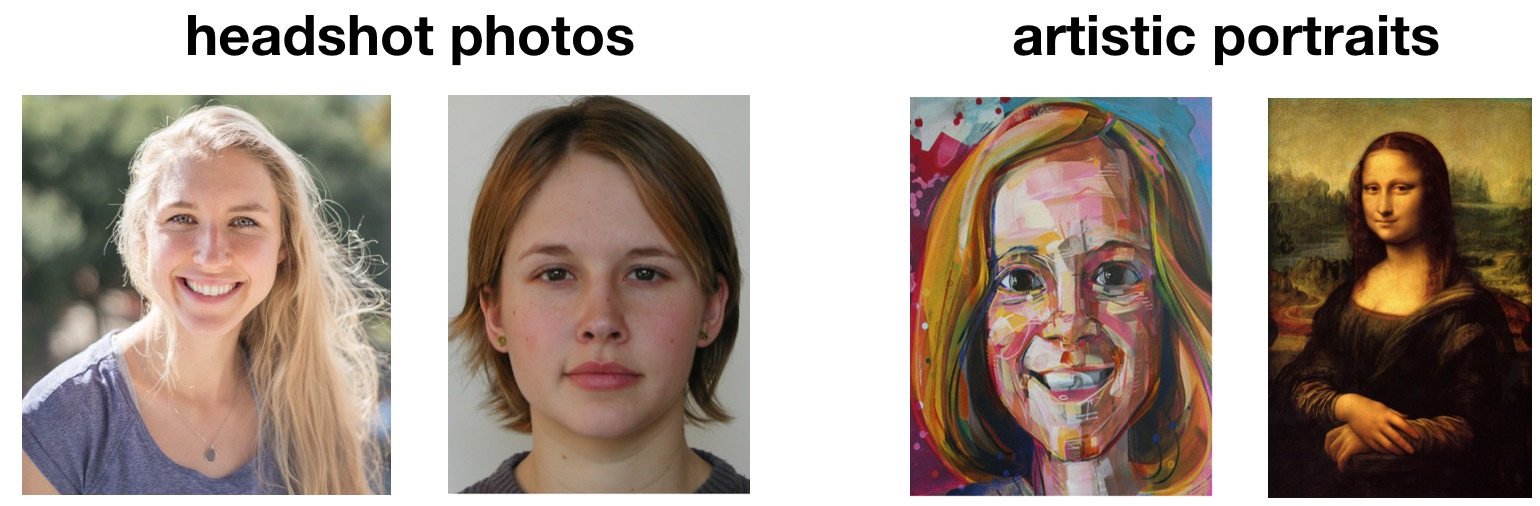
\includegraphics[width=.6\textwidth]{example_images2.jpg}
    \caption{Examples of headshot photographs and artistic portraits} \label{fig:examples}
  \end{center}
\end{figure} 

\section{ Methods }

Replacing an artistic face with a photographed face requires three main steps. First, we crop both faces, identify facial landmarks in each image, and warp the artistic face to align with the photographed face. This step is required for the portrait NST. Second, we generate a new image by performing portait-specific NST using the warped artistic image and the cropped photographed face. Third, we inpaint this new image into the original artistic photo. 

\subsection{Face alignment}

First, to align the artistic face with the photographed face, we cropped images to only contain faces by implementing an open-source face recognition from the OpenCV package \cite{opencv_library}. Following the procedure detailed in the Medium blogpost \cite{Medium}, we used a pre-trained Haar Feature-based Cascade Classifier to detect the bounding box of the face (Figure 2A-B). Second, we detected 68 prominent landmarks on both faces using the dlib face detection and landmark identification package \cite{dlibgit}, \cite{dlib09}, following the implementation in \cite{opencvImplement} (Figure 2C). We also added 8 landmarks around the boundary of the image. Briefly, the dlib landmark identification is performed via a cascade of regressors, where each regressor tries to learn the location of landmark points based on previous iterations. This model was trained on the Helen dataset, which contains 2000+ labeled faces \cite{Helen}. Third, we use an OpenCV package to compute the Delaunay triangles between all the points (Figure 2D), \cite{opencvImplement}. Here, triangulation is the process by which an image is segmented into triangles, such that landmark points form the vertex of the triangles. In Delaunay triangulation, the triangle lines are chosen such that no point is inside the circumcircle of any triangle \cite{dt}. Fourth, we warped the artistic photo to the pose of the photographed image by warping each triangle in the artistic image to match the corresponding triangle position in the photographed image (Figure 2E). This procedure is implemented via code adapted from \cite{opencvImplement}. Briefly, each artistic image triangle is put through an affine transform that will warp it into the shape of the corresponding triangle in the photograph image. This warped triangle is then replaced, via a masking and cloning procedure, into a new, warped image of the artistic face.

\begin{figure}[H]
  \begin{center}
    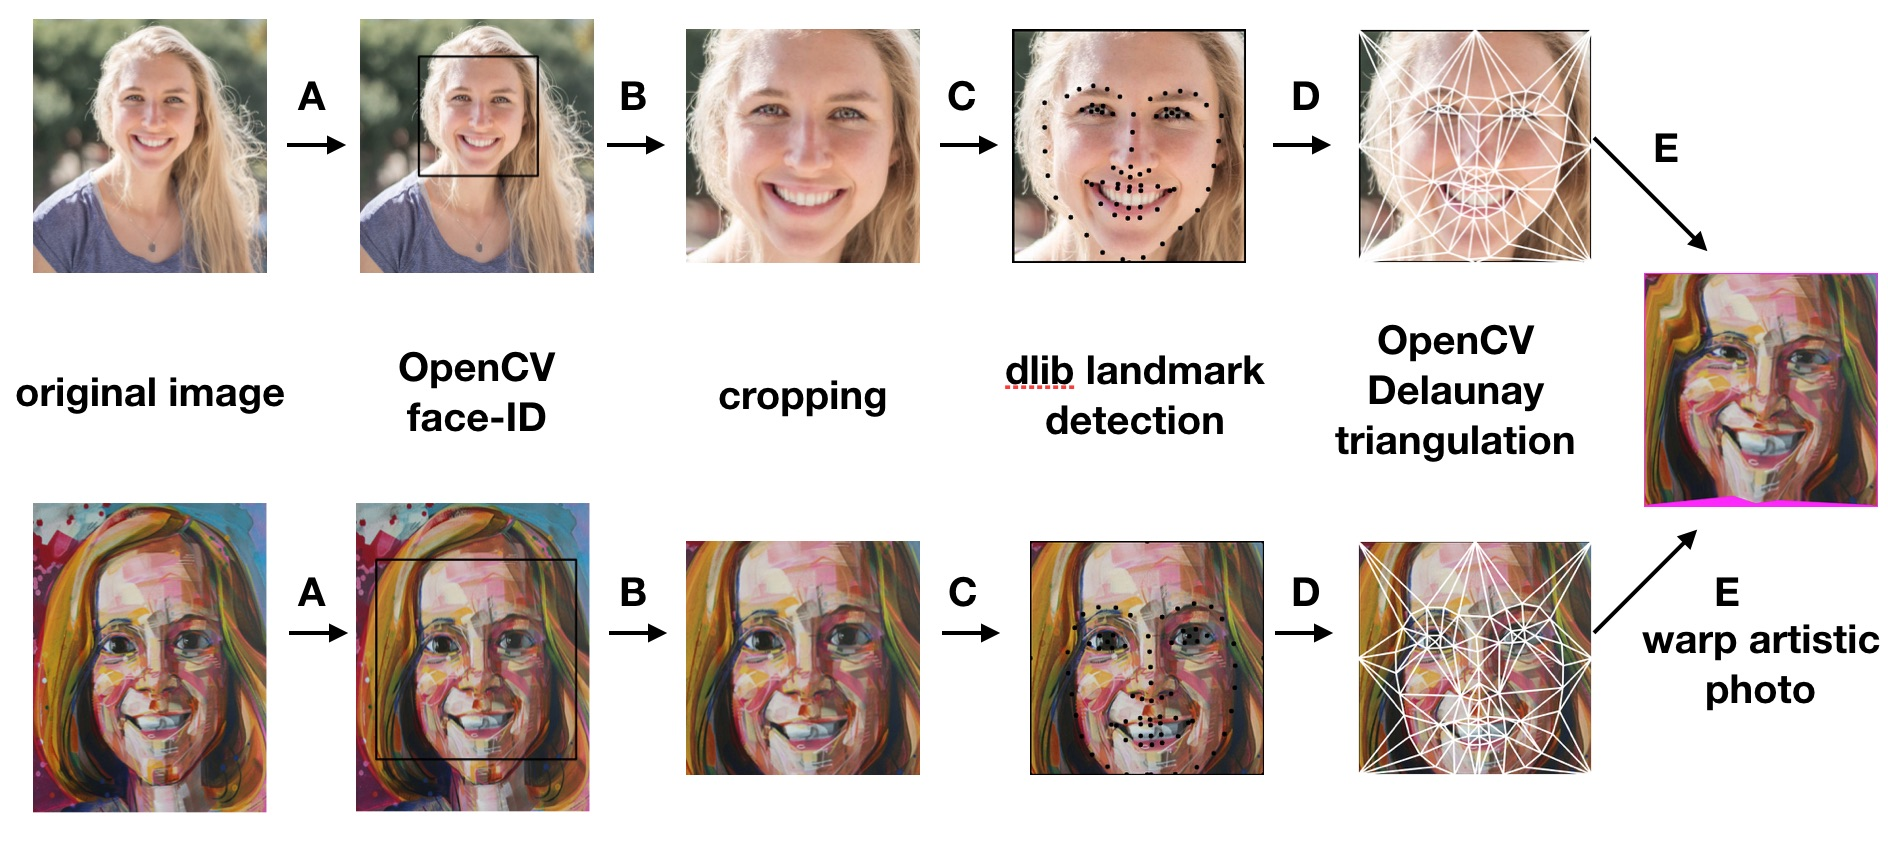
\includegraphics[width=0.8\textwidth]{phase_one_pipeline.jpg}
    \caption{Analysis pipeline for warping artistic portrait into the pose of the photographed face} \label{fig:examples}
  \end{center}
\end{figure} 


\subsection{Portrait Neural Style Transfer}

In the original implementation of NST, an image is learned via an optimization procedure in which the style-activations of the learned image attempt to match the style-activations of the style image, while the content-activations of the learned image attempt to match the content-activations of the content image. In our main implementation of portrait NST, we adapt the code presented in the Coursera course to reflect critical aspects of the model implemented in \cite{selim2016painting}, as well using code from the book by Gulli et al \cite{Gulli}. In particular, we use several layers to compute the cost function, we use max-pooling instead of average-pooling, and most importantly, we compute a "gains map" that influences the content cost function. In particular, the content cost function is given by: $J_{content}(C,G) = \sum_l  \frac{\lambda_l }{4n_Hn_Wn_H} \sum_{ij} ( A_{ij}^{(l)}(G) - A_{ij}^{(l)}(C)*G_{l}^{clamped})^2$, where $G$ corresponds to the generated image, $C$ corresponds to the content image (the cropped photograph face), and A^{(l)}(X)$ are the activations of layer $l$ of a pre-trained VGG-19 network with the image X as input (with the cost function computed over all $ij$ indices). Following \cite{selim2016painting}, we define $G_{l}^{clamped}$ as: $ G_{l}^{clamped} = \mathrm{max}\Big(\mathrm{min}\Big(\frac{A(S)}{A_l(C) + \epsilon},g_{max}\Big),g_{min}\Big)$, where $S$ corresponds to the style image (the warped artistic face). Similar to what is presented in the Coursera course, we use the following style content function: $J_{style}(S,G) = \sum_l \frac{\lambda_l }{(2n_Hn_Wn_H)^2} \sum_{ij} ( B_{ij}^{(l)}(S) - B_{ij}^{(l)}(G))^2$, where $B^{(l)}(S)$ Gram matrix of activations of a layer $l$ when the style image is pushed through (and $B^{(l)}(G)$ is defined similarly for the generated image G). To learn our generated image, we find the image that minimizes the following loss function: $J(G)=\alpha J_{content}(C,G)+\beta J_{style}(S,G)$, where $\alpha$ and $\beta$ are hyper-parameters that we choose. To implement this, we appropriately altered (and re-packaged) the code we implemented for the NST homework assignment, such that the new content cost function was implemented. Specifically, we used an Adam optimizer, and we trained the model for 500-1500 iterations. Importantly, we also changed the VGG model so that max-pooling was used (following \cite{selim2016painting}). In addition, we compared our implementation to another implementation we found at \cite{NeuralStyleTranferGithub}, which is an extended open-source implementation of NST as described in \cite{gatys2015neural} which incorporates a number of additions such as color, content and style masks as well as a number of other additions. 

\subsection{Face replacement}

Once the new image was generated, we then had to replace the original artistic face with the new image. To do this, we first identified the 68 dlib facial landmarks, and then identified the convex hull of these points. We then identified their Delaunay triangles using the same procedure as described above (Figure 3A-B). Then, as above, we warped each triangle by computing an affine transformation until each triangle in the artistic face was replaced (Figure 3C-D). We then implemented a seamless cloning using \cite{opencvImplement}, which will match the colors and blend the edges of the image (Figure 3E). Lastly, we replaced the original bounding box of the face in the artistic photo with the blended image (Figure 3F).  

\begin{figure}[H]
  \begin{center}
    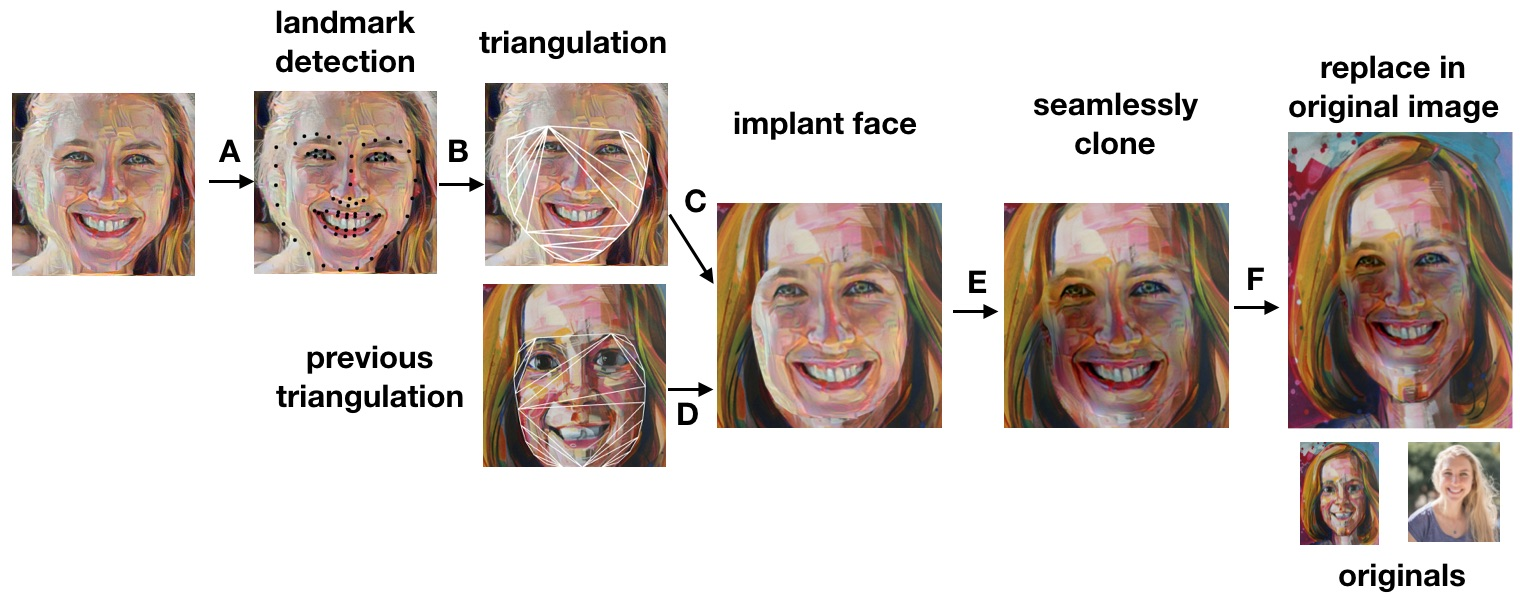
\includegraphics[width=0.8\textwidth]{post_nst_pipeline2.jpg}
    \caption{Analysis pipeline used to implant styled photograph phase into artistic portrait} \label{fig:examples}
  \end{center}
\end{figure} 

\section{Experiments/Results/Discussion}

Figure 4 shows a summary of our results. Overall, we had varying degrees of success in the portrait NST and the second stage of face morphing. The best result for the NST was achieved via using the open-source implementation of NST \cite{NeuralStyleTranferGithub}. We completed an extensive hyper-parameter search to improve the quality of the image. In this project, we focused on varying the parameters $\alpha$, $\beta$, the number of style layers, the weights between style layers, the presence/absence of the gains map, the number of iterations. Each result was then independently scored twice on a 10-point scale, after which we took the average as our final quantitative measure. While we used this metric to evaluate results, we mostly focused qualitative feedback for each of our experiments (as was done in Selim et al., 2016).

The order of our parameter search was initialized along permutations with the following values: $\alpha \in \{1,10,000\}$, $\beta \in \{1,10,000\}$, number of style layers (2 style layers (Conv$3_1$, Conv4$_1$) or 5 style layers (Conv$\mathrm1_1$, Conv$2_1$,Conv$3_1$, Conv$4_1$,Conv$5_1$)), number of content layers, 1 content layer (Conv$4_1$)  or 2 content layers (Conv$3_1$, Conv$4_1$)), number of iterations (100-800), the weights between style and content layers (equal vs. ascending), and the presence or absence of gains map. Example outputs of this parameter search are shown in Figure 4B. 

Overall, we first analysed the iterations needed for our loss function to converge, and observed that the optimization converged for all experiments within 300 iterations (Figure 4A). Second, we found that making $\alpha$ too large resulted in large facial distortions where the content of the style image blended over, while having $\beta$ equally as large did not introduce such distortions. Interestingly, we did not observe strong effects in changing either the weights or layers included in the style cost. When we including the layers in the content cost there was a slight observable difference in the types of style artifacts that were introduced with a preference for using 2 content layers. However, in regimes when $\alpha$ introduced distortions, removing the gain map removed said distortions. 

We also focused on varying the ways in which we warped and in-painted the image. First, we initially tried warping the headshot photo to match the pose of the artistic face, but this was not successful. Second, we tried various methods of in-painting the image. In particular, we varied the number of landmark points used to warp the image - we tried the convex hull (presented in the methods), along with using all landmark points to warp the image (Figure 4C). However, the latter method substantially distorted the face, removing the identifiable features.
 

\begin{figure}[H]
  \begin{center}
    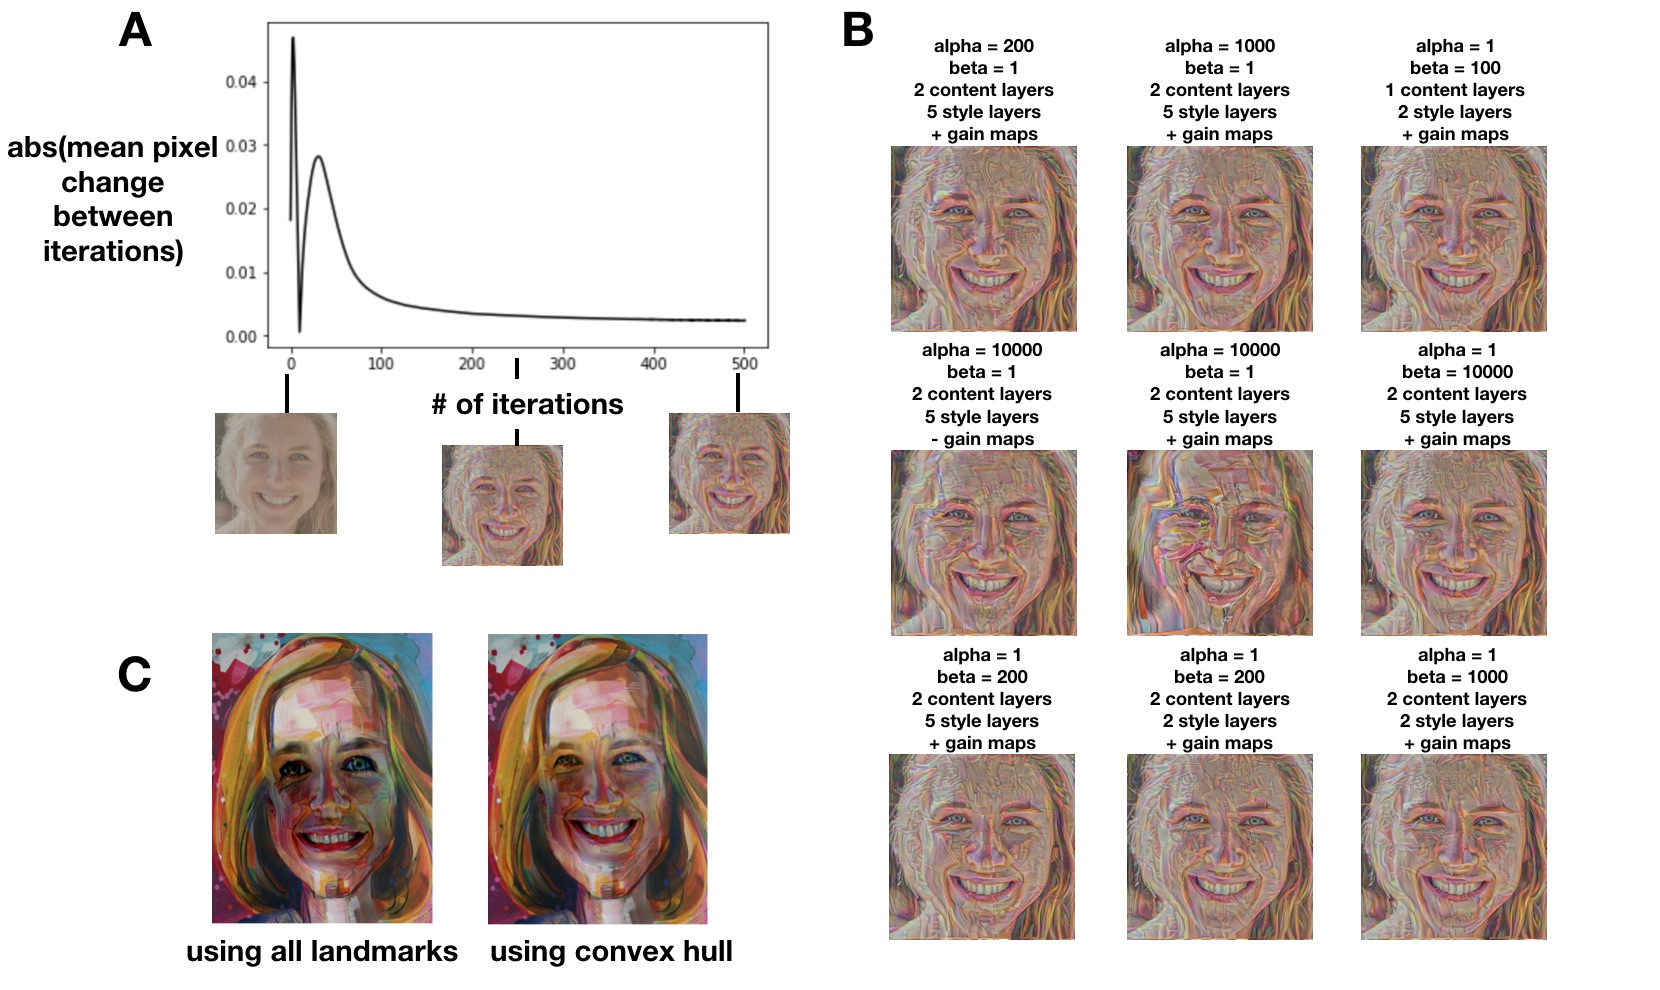
\includegraphics[width=0.8\textwidth]{results2.jpg}
    \caption{Summary of our hyperparameter search. A. Images don't change after 300 iterations. B. Selection of results from hyperparameter search. C. Result from using different methods in in-painting face.} \label{fig:examples}
  \end{center}
\end{figure} 


\section{Conclusion/Future Work}

In this project, we combined face-alignment and face-warping with portrait neural style transfer techniques in order to replace the face in an artistic painting with the face from a headshot photo. In order to do this, we identified candidate images, identified faces and warped the artistic portrait face, performed portrait NST, and then replaced the artisitic face with the newly styled face. We compared our results of the portrait NST with that from an open-source implementation of Gatys et al, 2015 \cite{NeuralStyleTranferGithub}, and found subpar results. We tried a number of different avenues in order to improve our image quality, including extensive hyperparameter searches, although without much success.  

If we had more time or resources, we would explore more of the hyper-parameters space for the portrait NST. Our implementation returns images with lower quality than reported, even though we believe that we are implementing it correctly. It is possible that details within the VGG-19 model differ, or that we need to use different hyperparameters. In addition, in order to improve the last step of the face-replacement, we would identify 3d landmarks of the face that determine the pose, and find the proper rotation and alignment to better inpaint the styled face into the artistic image. We would also work to improve the cloning so that the color isn't altered in the final image. 


\newpage

\section{Contributions and Code}
Kiah Hardcastle implemented the face warping and face replacement. Julie Makelberge implemented the Neural Style Transfer section. Both contibuted to the project write-up and poster, as well as developing high-level ideas and helping with trouble-shooting. We both feel we contributed equally to this project. All code for this project can be found on: \url{https://github.com/khardcastle/face-in-art}.

\section{Acknowledgments}
We thank Andrew Ng and Kian Katanforoosh for teaching us the techniques used in this project, and to our project TA Kaidi Cao for guiding us towards workable solutions for our problem and pointing us to relevant literature.


\small

\bibliography{References}
\bibliographystyle{plain}

\end{document}